\documentclass[aspectratio=169,10pt]{beamer}

\usepackage[utf8]{inputenc}
\usepackage{lmodern}
\usepackage{booktabs}
\usepackage{xcolor}
\usepackage{colortbl}
\usepackage{graphicx}
\usepackage{array}
\usepackage{hyperref}
\usepackage{tikz}

\usetheme{metropolis}

% ── King Khalid University colour palette ─────────────────────────
%   kkuGreen     #045531  — deep institutional green (from the logo)
%   kkuGreenDark #023922  — shading for accents / backgrounds
%   kkuGold      #C9A959  — KKU gold for highlights and rules
%   kkuGoldLight #EDDBA6  — soft gold for block fills
%   kkuInk       #1a1a1a  — body text
%   kkuSubtle    #6b7280  — secondary / caption text
\definecolor{kkuGreen}{HTML}{045531}
\definecolor{kkuGreenDark}{HTML}{023922}
\definecolor{kkuGold}{HTML}{C9A959}
\definecolor{kkuGoldLight}{HTML}{EDDBA6}
\definecolor{kkuInk}{HTML}{1A1A1A}
\definecolor{kkuSubtle}{HTML}{6B7280}

% Apply palette to the metropolis theme
\setbeamercolor{normal text}{fg=kkuInk, bg=white}
\setbeamercolor{alerted text}{fg=kkuGold}
\setbeamercolor{example text}{fg=kkuGreen}
\setbeamercolor{structure}{fg=kkuGreen}
\setbeamercolor{frametitle}{fg=white, bg=kkuGreen}
\setbeamercolor{progress bar}{fg=kkuGold, bg=kkuGoldLight}
\setbeamercolor{title separator}{fg=kkuGold}
\setbeamercolor{progress bar in head/foot}{fg=kkuGreen, bg=kkuGoldLight}
\setbeamercolor{progress bar in section page}{fg=kkuGold, bg=kkuGoldLight}
\setbeamercolor{section title}{fg=kkuGreen}
\setbeamercolor{block title}{fg=white, bg=kkuGreen}
\setbeamercolor{block body}{fg=kkuInk, bg=kkuGoldLight!35}
\setbeamercolor{block title alerted}{fg=white, bg=kkuGold}
\setbeamercolor{block body alerted}{fg=kkuInk, bg=kkuGoldLight}
\setbeamercolor{block title example}{fg=white, bg=kkuGreenDark}
\setbeamercolor{block body example}{fg=kkuInk, bg=kkuGoldLight!20}
\setbeamercolor{itemize item}{fg=kkuGreen}
\setbeamercolor{itemize subitem}{fg=kkuGold}
\setbeamercolor{enumerate item}{fg=kkuGreen}

\metroset{block=fill, progressbar=frametitle, numbering=fraction, sectionpage=progressbar}

% Legacy colour aliases kept for existing \textcolor{...} calls.
\definecolor{ok}{HTML}{2ecc71}
\definecolor{alert}{HTML}{e74c3c}
\definecolor{subtle}{HTML}{7f8c8d}
\definecolor{kku}{HTML}{045531}

% Small logo in the footer of every non-title slide.
\setbeamertemplate{frame footer}{%
  
\includegraphics[height=3.2mm]{figures/misc/kku-logo.png}%
  \hspace{0.4em}\small King Khalid University \textbar{} College of Computer Science
}

\title{Genetic Mutation Detection Using Machine Learning}
\subtitle{A Rigorous Baseline with Paralog-Aware Evaluation \\ and Gene-Level Constraint Features}
\author[Team KKU-CS]{
  Rayan Saleh AlShahrani \and Zahran Ali AlZahrani \and Saad Saleh Saad \\[0.2em]
  Eyad Hassan AlSheri \and Khalid Hamdan Zuhair \and Abdullah Saeed Ali Asiri
}
\institute[KKU]{College of Computer Science \\ King Khalid University \\[0.3em]
\small Supervised by Dr.~Maaki Abubakr}
\date{Academic Year 2025/2026 (Semester~2)}

% ───────────────── KKU-branded title page ─────────────────
\setbeamertemplate{title page}{%
  \begin{tikzpicture}[remember picture, overlay]
    % top coloured band
    \fill[kkuGreen] (current page.north west) rectangle ([yshift=-2.2cm]current page.north east);
    \node[anchor=center] at ([yshift=-1.1cm]current page.north)
      {
\includegraphics[height=1.6cm]{figures/misc/kku-logo.png}};
    % bottom gold accent
    \fill[kkuGold] ([yshift=1.2cm]current page.south west) rectangle (current page.south east);
  \end{tikzpicture}%
  \vspace*{2.4cm}
  \begin{center}
    {\LARGE\bfseries\color{kkuGreen}\inserttitle\par}
    \vspace{0.4cm}
    {\large\color{kkuInk}\insertsubtitle\par}
    \vspace{1.2cm}
    {\small\color{kkuInk}\insertauthor\par}
    \vspace{0.7cm}
    {\small\color{kkuSubtle}\insertinstitute\par}
    \vspace{0.6cm}
    {\footnotesize\color{kkuSubtle}\insertdate\par}
  \end{center}
}

\begin{document}

% ───────────────────────────── SLIDE 1 ─────────────────────────────
\maketitle

% ───────────────────────────── SLIDE 2 ─────────────────────────────
\begin{frame}{Agenda}
  \begin{columns}[t]
    \column{0.5\linewidth}
    \textbf{Part I -- The problem}
    \begin{enumerate}
      \item Introduction (3 slides)
      \item Related works (3 slides)
      \item Contribution (1 slide)
    \end{enumerate}

    \textbf{Part II -- The pipeline}
    \begin{enumerate}\setcounter{enumi}{3}
      \item Proposed system flowchart
      \item Part~1: Preprocessing
      \item Part~2: Training + leakage audit
      \item Part~3: Evaluation + external validation
    \end{enumerate}

    \column{0.5\linewidth}
    \textbf{Part III -- System Analysis}
    \begin{enumerate}\setcounter{enumi}{7}
      \item Requirements + 6 UML diagrams
      \item Interface
      \item Implementation (stack, code, CI)
    \end{enumerate}

    \textbf{Part IV -- Results}
    \begin{enumerate}\setcounter{enumi}{10}
      \item Comparison with prior work
      \item Conclusion + future work
    \end{enumerate}
  \end{columns}
\end{frame}

% ═════════════════ PART 1: INTRODUCTION ═════════════════
\section{Introduction}

% ───────────── SLIDE 3 ─────────────
\begin{frame}{What is a missense variant?}
  \begin{itemize}
    \item A point mutation that changes one amino acid in a protein.
    \item \alert{Most common} coding variant in the human genome.
    \item A clinically-important minority cause disease; the majority
          are benign.
    \item Distinguishing the two is the central problem of
          \emph{clinical genetics}.
  \end{itemize}
  \vspace{0.8em}
  \begin{block}{The scale problem}
    \centering
    \large Exome sequencing generates $\sim$\textbf{20{,}000} variants per
    patient \\ Human curation bandwidth: $\sim$a few hundred per day
  \end{block}
\end{frame}

% ───────────── SLIDE 4 ─────────────
\begin{frame}{Why it's hard}
  Three well-known failure modes in prior work:
  \vspace{0.4em}
  \begin{enumerate}
    \item \textcolor{alert}{Definitional circularity}\\
          Features derived from the label (e.g.\ \texttt{is\_common})
          inflate metrics.
    \item \textcolor{alert}{Meta-predictor contamination}\\
          Using REVEL/CADD as features in a ClinVar benchmark.
    \item \textcolor{alert}{Paralog leakage}\\
          KRT1 in train + KRT14 in test $\Rightarrow$ 80\% sequence
          identity $\Rightarrow$ model ``saw'' most of the test.
  \end{enumerate}
  \vspace{0.4em}
  \begin{alertblock}{Consequence}
    High benchmark numbers do not survive \textbf{external validation}.
  \end{alertblock}
\end{frame}

% ───────────── SLIDE 5 ─────────────
\begin{frame}{Project objectives}
  \begin{enumerate}
    \item Assemble a clean, paralog-disjoint corpus of $195$k missense
          variants.
    \item Eliminate three specific leakage sources.
    \item Train and calibrate a defensible baseline.
    \item Re-score published tools on our test split.
    \item Evaluate externally on \textsc{denovo-db}.
    \item Prove orthogonality of protein-language-model signal
          (zero-shot ESM-2).
    \item Publish everything: code, tests, Docker, $10$ narrative
          notebooks, Streamlit demo, academic report.
  \end{enumerate}
\end{frame}

% ═════════════════ PART 2: RELATED WORKS ═════════════════
\section{Related Works}

% ───────────── SLIDE 6 ─────────────
\begin{frame}{Classical tools (2003--2010)}
  \small
  \centering
  \begin{tabular}{@{} l r l p{4cm} @{}}
    \toprule
    Tool & Year & Approach & Limitation \\
    \midrule
    SIFT          & 2003 & conservation only              & no AA chemistry \\
    PolyPhen-2    & 2010 & conservation + chemistry + struct. & HumDiv overlaps ClinVar \\
    \bottomrule
  \end{tabular}
  \vspace{0.8em}
  \begin{itemize}
    \item Access: Ensembl VEP REST, instant.
    \item Coverage: $\sim$93--96\% of our test variants.
    \item \alert{Threshold design:} SIFT picks 0.05 arbitrarily.
  \end{itemize}
\end{frame}

% ───────────── SLIDE 7 ─────────────
\begin{frame}{Gradient-boosted ensembles (2016--2024)}
  \small
  \centering
  \begin{tabular}{@{} l r l p{4.3cm} @{}}
    \toprule
    Tool    & Year & Approach & Limitation \\
    \midrule
    REVEL   & 2016 & RF ensemble of 13 tools     & input tools ClinVar-trained \\
    CADD    & 2019 & logistic/RF simulated null   & scores not calibrated \\
    VARITY  & 2021 & XGBoost + noise weighting    & gene-level split only \\
    MAGPIE  & 2024 & gradient boosting            & paralog status undocumented \\
    \bottomrule
  \end{tabular}
  \vspace{0.8em}
  \begin{itemize}
    \item All sit above 0.92 ROC-AUC on their own benchmarks.
    \item None report a \emph{like-for-like} external test.
    \item None publish bootstrap CIs on every metric.
  \end{itemize}
\end{frame}

% ───────────── SLIDE 8 ─────────────
\begin{frame}{Protein language models (2021--2023)}
  \small
  \centering
  \begin{tabular}{@{} l r p{7cm} @{}}
    \toprule
    Tool           & Year & Core idea \\
    \midrule
    EVE            & 2021 & Variational auto-encoder per gene ($\sim$3k genes) \\
    ESM-1b / 2 (zero-shot) & 2023 & Masked-AA log-likelihood ratio from 250M sequences \\
    AlphaMissense  & 2023 & Structural PLM calibrated on ClinVar \\
    \bottomrule
  \end{tabular}
  \vspace{0.8em}
  \begin{block}{Why the PLM wave matters}
    ESM-2 is fully unsupervised $\Rightarrow$ provably
    \textbf{uncontaminated} by ClinVar.
    Our Phase~2.1 integrates it as a training-time feature.
  \end{block}
\end{frame}

% ═════════════════ PART 3: CONTRIBUTION ═════════════════
\section{Contribution}

% ───────────── SLIDE 9 ─────────────
\begin{frame}{What we contribute}
  \begin{enumerate}
    \item \textbf{Transparent leakage audit} with
          before-and-after numbers (PR-AUC $0.955 \rightarrow 0.838$).
    \item \textbf{Like-for-like re-scoring} of three published
          baselines on our own paralog-disjoint test.
    \item \textbf{External validation on \textsc{denovo-db}} with
          pre/post gnomAD-constraint decomposition.
    \item \textbf{Zero-shot ESM-2 proof-of-concept} under rank-fusion.
    \item \textbf{Fully reproducible code base}: $158$ tests,
          CI-enforced leakage gate, pinned deps, Docker, Streamlit
          demo, LaTeX report.
  \end{enumerate}
  \vspace{0.5em}
  \centering
  \small \url{github.com/RayanAlDwlah/Genetic-Mutation-Detection-project}
\end{frame}

% ═════════════════ PART 4: PROPOSED SYSTEM ═════════════════
\section{Proposed System}

% ───────────── SLIDE 10 ─────────────
\begin{frame}{Pipeline -- three parts}
  \centering
  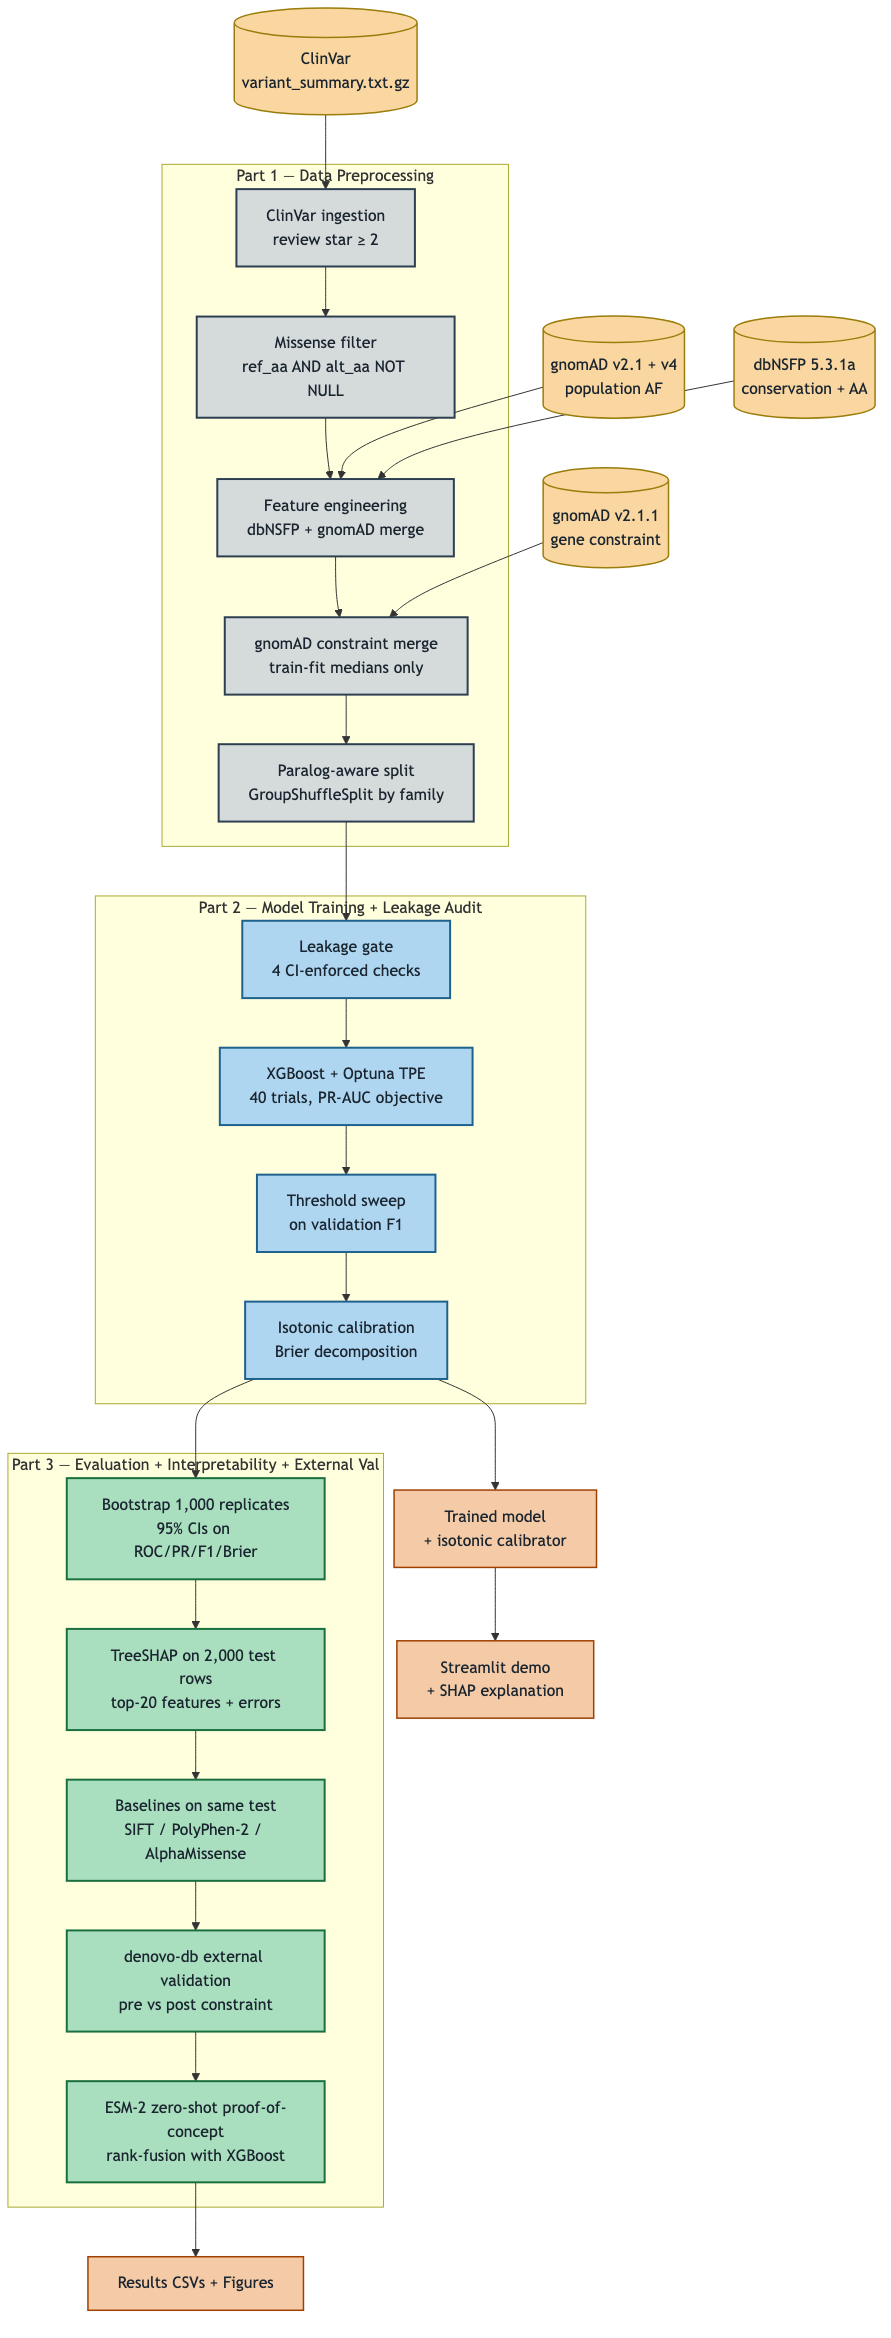
\includegraphics[width=\linewidth,height=0.78\textheight,keepaspectratio]{figures/flowcharts/01_pipeline_3parts.png}
\end{frame}

% ───────────── SLIDE 11 ─────────────
\begin{frame}{Part 1 -- Data preprocessing (1/3)}
  \textbf{Sources:}
  \begin{itemize}
    \item \textsc{ClinVar} -- pathogenic / benign labels (review star $\geq 2$)
    \item \textsc{gnomAD} v2.1 + v4 -- allele frequency, AC, AN
    \item \textsc{dbNSFP} 5.3 -- conservation + AA chemistry + Pfam
    \item \textsc{gnomAD} v2.1.1 -- gene-level constraint (pLI, LOEUF, mis\_z)
  \end{itemize}
  \vspace{0.4em}
  \textbf{Join key:} canonical \texttt{chr:pos:ref:alt} on \textsc{GRCh38}.
\end{frame}

% ───────────── SLIDE 12 ─────────────
\begin{frame}{Part 1 -- Data preprocessing (2/3)}
  \textbf{The critical filter}
  \vspace{0.3em}
  \begin{block}{Missense-only}
    \centering Drop every row with null \texttt{ref\_aa} OR null
    \texttt{alt\_aa} $\Rightarrow$ \textbf{remove $\sim$88{,}000
    non-missense rows.}
  \end{block}
  \vspace{0.3em}
  \begin{itemize}
    \item Pre-audit: 64\% of pathogenic rows had null AA fields!
    \item Model was learning ``null AA $\Rightarrow$ pathogenic''
    \item Fix alone drops PR-AUC $0.955 \rightarrow 0.819$
          (the single biggest audit finding)
  \end{itemize}
\end{frame}

% ───────────── SLIDE 13 ─────────────
\begin{frame}{Part 1 -- Data preprocessing (3/3): paralog-aware split}
  \begin{itemize}
    \item Plain gene-level split: 52\% of prefix families (ZNF*, SLC*,
          KRT*, TMEM*) shared between train and test.
    \item Fix: \textbf{family-level} split via
          \texttt{assign\_gene\_family} (16 regex patterns +
          trailing-digit fallback).
    \item Result: 15{,}479 genes $\to$ 7{,}851 families, \textbf{zero}
          shared across splits, enforced by CI.
  \end{itemize}
\end{frame}

% ───────────── SLIDE 14 ─────────────
\begin{frame}{Part 2 -- Leakage audit (1/4)}
  \begin{block}{Four CI-enforced invariants}
    \vspace{0.3em}
    \begin{enumerate}
      \item No banned features (\texttt{is\_common, chr, ref, alt}) in
            the training matrix.
      \item 100\% missense-only rows in training split.
      \item Zero shared gene families across train/val/test.
      \item Pathogenic-rate gap $<$ 0.08 across splits.
    \end{enumerate}
  \end{block}
  \vspace{0.4em}
  \textbf{Every push to \texttt{main} runs the four checks.} \\
  A failure blocks the merge.
\end{frame}

% ───────────── SLIDE 15 ─────────────
\begin{frame}{Part 2 -- Five-stage leakage journey (2/4)}
  \centering
  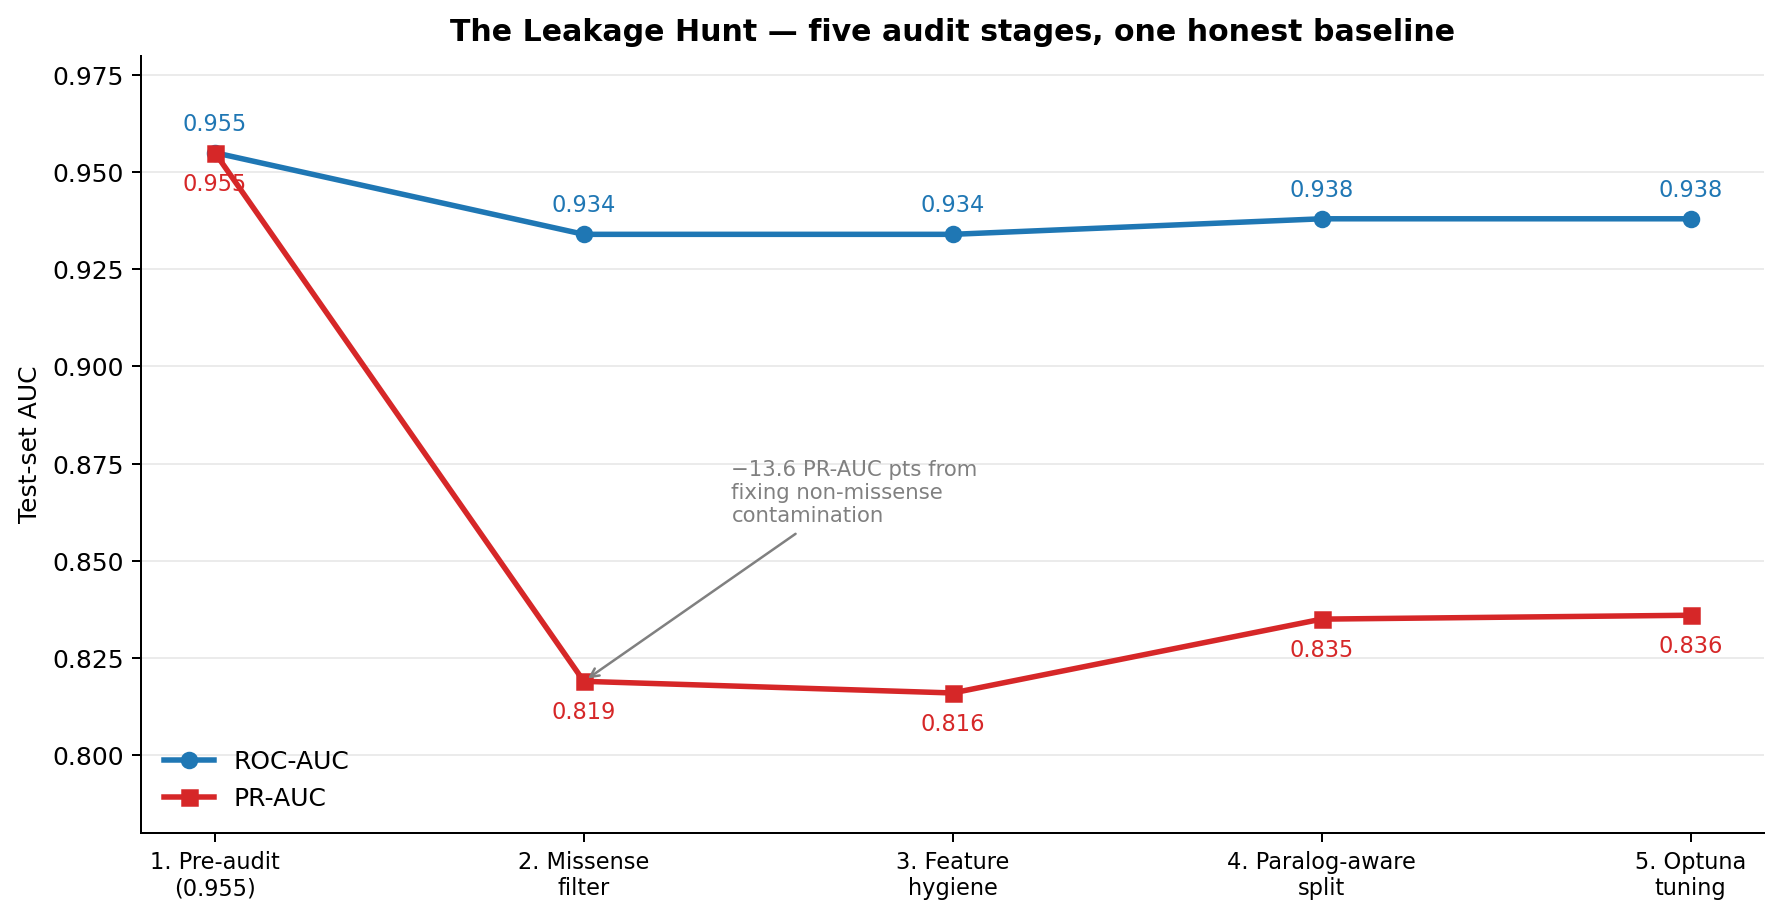
\includegraphics[width=\linewidth,height=0.78\textheight,keepaspectratio]{figures/scientific/leakage_journey.png}
\end{frame}

% ───────────── SLIDE 16 ─────────────
\begin{frame}{Part 2 -- Model + calibration (3/4)}
  \textbf{Model}: XGBoost, Optuna TPE with multivariate grouping, $40$
  trials, PR-AUC objective, median pruner after 200 rounds.

  \textbf{Calibration}: isotonic regression fit on validation,
  evaluated via Murphy's Brier decomposition:
  $$\text{Brier} = \text{Reliability} - \text{Resolution} + \text{Uncertainty}$$

  \vspace{0.5em}
  \small
  \centering
  \begin{tabular}{@{} l r r r r @{}}
    \toprule
    & Brier & Reliability & Resolution & ECE \\
    \midrule
    Raw      & 0.0876 & 0.00543 & 0.1055 & 0.054 \\
    Platt    & 0.0834 & 0.00114 & 0.1055 & 0.029 \\
    \textbf{Isotonic} & \textbf{0.0826} & \textbf{0.00024} & 0.1053 & \textbf{0.011} \\
    \bottomrule
  \end{tabular}
  \vspace{0.3em}
  \begin{itemize}
    \item Resolution constant $\Rightarrow$ discrimination unchanged.
    \item Reliability drops $23\times$ $\Rightarrow$ calibration works.
  \end{itemize}
\end{frame}

% ───────────── SLIDE 17 ─────────────
\begin{frame}{Part 2 -- Reliability triptych (4/4)}
  \centering
  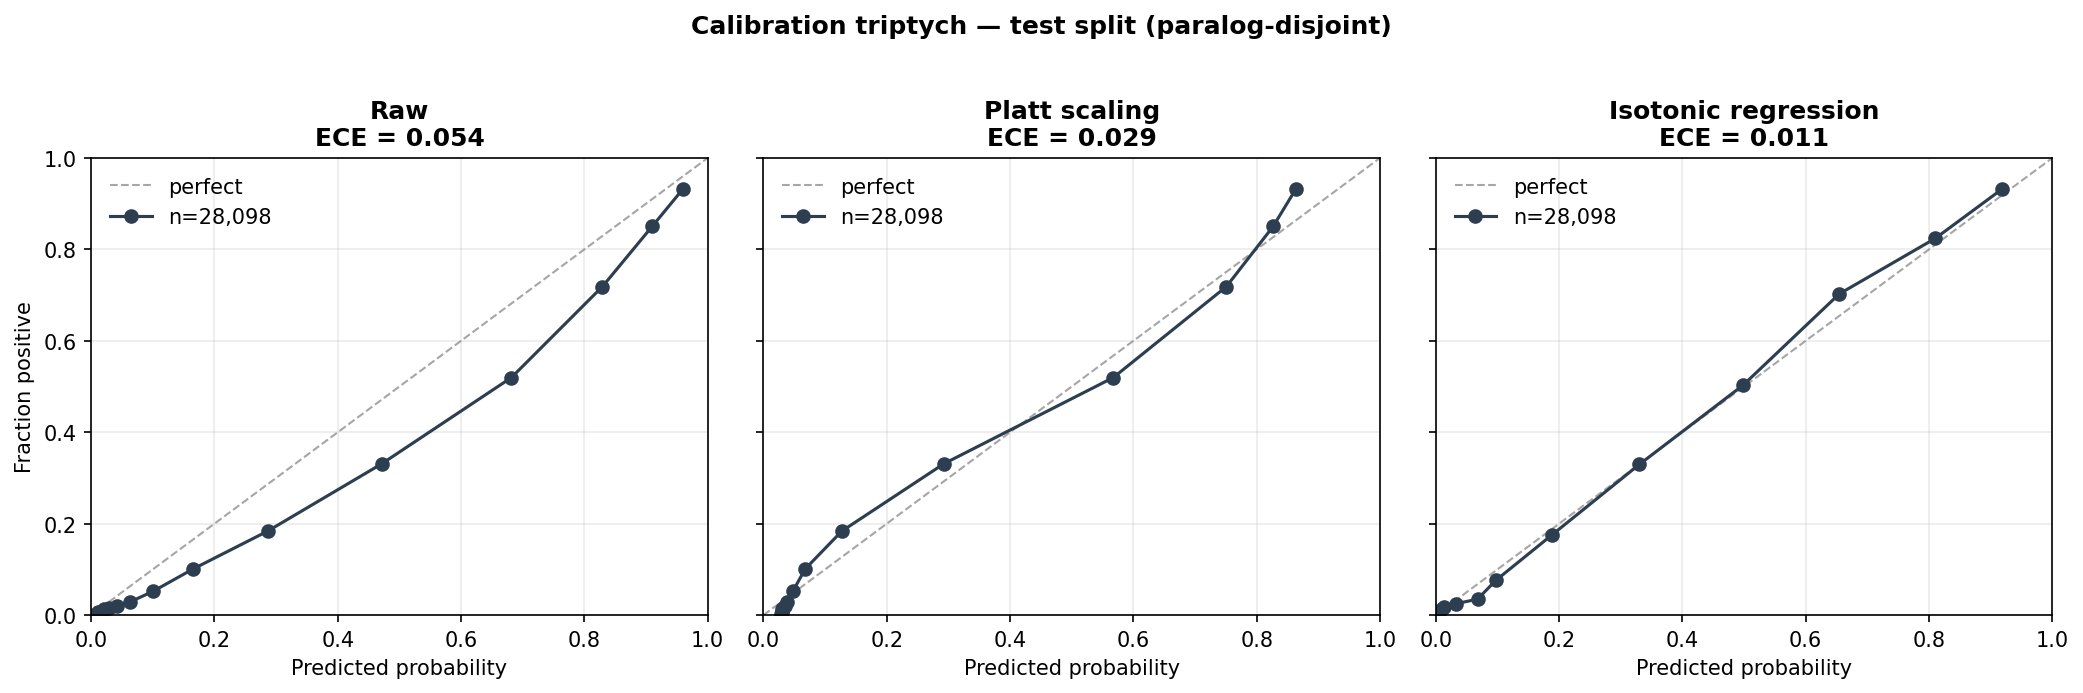
\includegraphics[width=\linewidth,height=0.8\textheight,keepaspectratio]{figures/scientific/calibration_triptych.png}
\end{frame}

% ───────────── SLIDE 18 ─────────────
\begin{frame}{Part 3 -- Headline results on test (1/3)}
  \centering
  \textbf{Test split (paralog-disjoint), 28{,}098 variants}
  \vspace{0.5em}
  \begin{tabular}{@{} l r @{}}
    \toprule
    Metric & Value (95\% CI) \\
    \midrule
    ROC-AUC              & 0.938 $[0.935, 0.941]$ \\
    PR-AUC               & 0.838 $[0.830, 0.846]$ \\
    F1                   & 0.775 \\
    Brier (calibrated)   & 0.083 \\
    ECE (calibrated)     & 0.011 \\
    \bottomrule
  \end{tabular}
  \vspace{0.5em}
  \begin{block}{}
    All CIs from $1{,}000$-replicate nonparametric bootstrap.
  \end{block}
\end{frame}

% ───────────── SLIDE 19 ─────────────
\begin{frame}{Part 3 -- SHAP interpretability (2/3)}
  \small
  \centering
  \begin{tabular}{@{} r l r @{}}
    \toprule
    Rank & Feature & mean $|$SHAP$|$ \\
    \midrule
    1 & phyloP100way\_vertebrate & 0.809 \\
    2 & AN (gnomAD allele number) & 0.532 \\
    \rowcolor{yellow!25}
    3 & \textbf{lof\_z (gnomAD constraint)} & 0.342 \\
    4 & alt\_aa\_P (Proline) & 0.304 \\
    5 & pfam\_domain & 0.284 \\
    \rowcolor{yellow!25}
    8 & \textbf{oe\_mis\_upper (gnomAD constraint)} & 0.189 \\
    \bottomrule
  \end{tabular}
  \vspace{0.5em}
  \begin{itemize}
    \item Two Phase~2.1 features at \#3 and \#8 $\Rightarrow$
          gene-level priors carry \textbf{orthogonal signal}.
    \item $326$ of $2{,}000$ test variants are confident errors
          ($16.3\%$).
    \item FN $= 264$, FP $= 62$ $\Rightarrow$ model misses hard
          pathogenic cases in low-conservation regions.
  \end{itemize}
\end{frame}

% ───────────── SLIDE 20 ─────────────
\begin{frame}{Part 3 -- External validation: denovo-db (3/3)}
  \small
  \centering
  \begin{tabular}{@{} l r l l @{}}
    \toprule
    Slice & $n$ & ROC-AUC (95\% CI) & PR-AUC (95\% CI) \\
    \midrule
    full (pre-constraint)      & 642 & 0.468 $[0.42, 0.52]$ & 0.761 \\
    full (post-constraint)     & 642 & \textbf{0.511} $[0.46, 0.56]$ & \textbf{0.790} \\
    \rowcolor{yellow!25}
    holdout (pre-constraint)   & 201 & 0.487 $[0.38, 0.58]$ & 0.789 \\
    \rowcolor{yellow!25}
    \textbf{holdout (post-constraint)} & 201 & \textbf{0.573} $[0.48, 0.67]$ & \textbf{0.838} \\
    \bottomrule
  \end{tabular}
  \vspace{0.6em}
  \begin{alertblock}{The headline}
    \centering
    On \textbf{unseen} gene families, ROC jumps from 0.487 (chance)
    to 0.573 --- gene-level priors close \textbf{half} the
    generalisation gap.
  \end{alertblock}
\end{frame}

% ═════════════════ PART 5: SYSTEM ANALYSIS & DESIGN ═════════════════
\section{System Analysis \& Design}

% ───────────── SLIDE 21 ─────────────
\begin{frame}{Functional + non-functional requirements}
  \textbf{Functional ($\times 8$):} ingestion, feature assembly,
  scoring, risk categorisation, feature attribution, batch mode,
  external reproduction, report regeneration.

  \vspace{0.5em}
  \textbf{Non-functional ($\times 7$):} performance ($<$100\,ms
  cache hit), reliability (seed-reproducible to $10^{-3}$),
  scalability ($10^{6}$ variants), usability (non-ML end user),
  maintainability (CI enforced), security (no PHI), reproducibility
  (Docker-replayable).

  \vspace{0.6em}
  \textbf{Traceability:} every requirement maps to at least one
  \texttt{src/} module and at least one pytest test case.
\end{frame}

% ───────────── SLIDE 22 ─────────────
\begin{frame}{UML 1/3: Use case + Class}
  \begin{columns}[t]
    \column{0.5\linewidth}
    \centering
    \textbf{Use case diagram}\\[0.3em]
    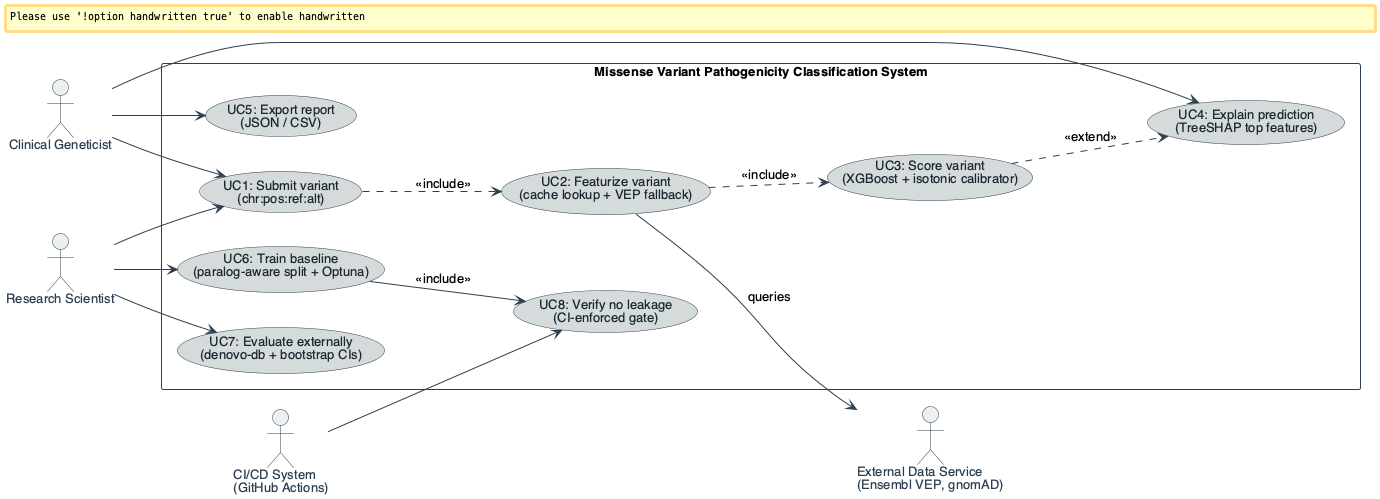
\includegraphics[width=\linewidth,height=0.78\textheight,keepaspectratio]{figures/uml/01_use_case.png}

    \column{0.5\linewidth}
    \centering
    \textbf{Class diagram}\\[0.3em]
    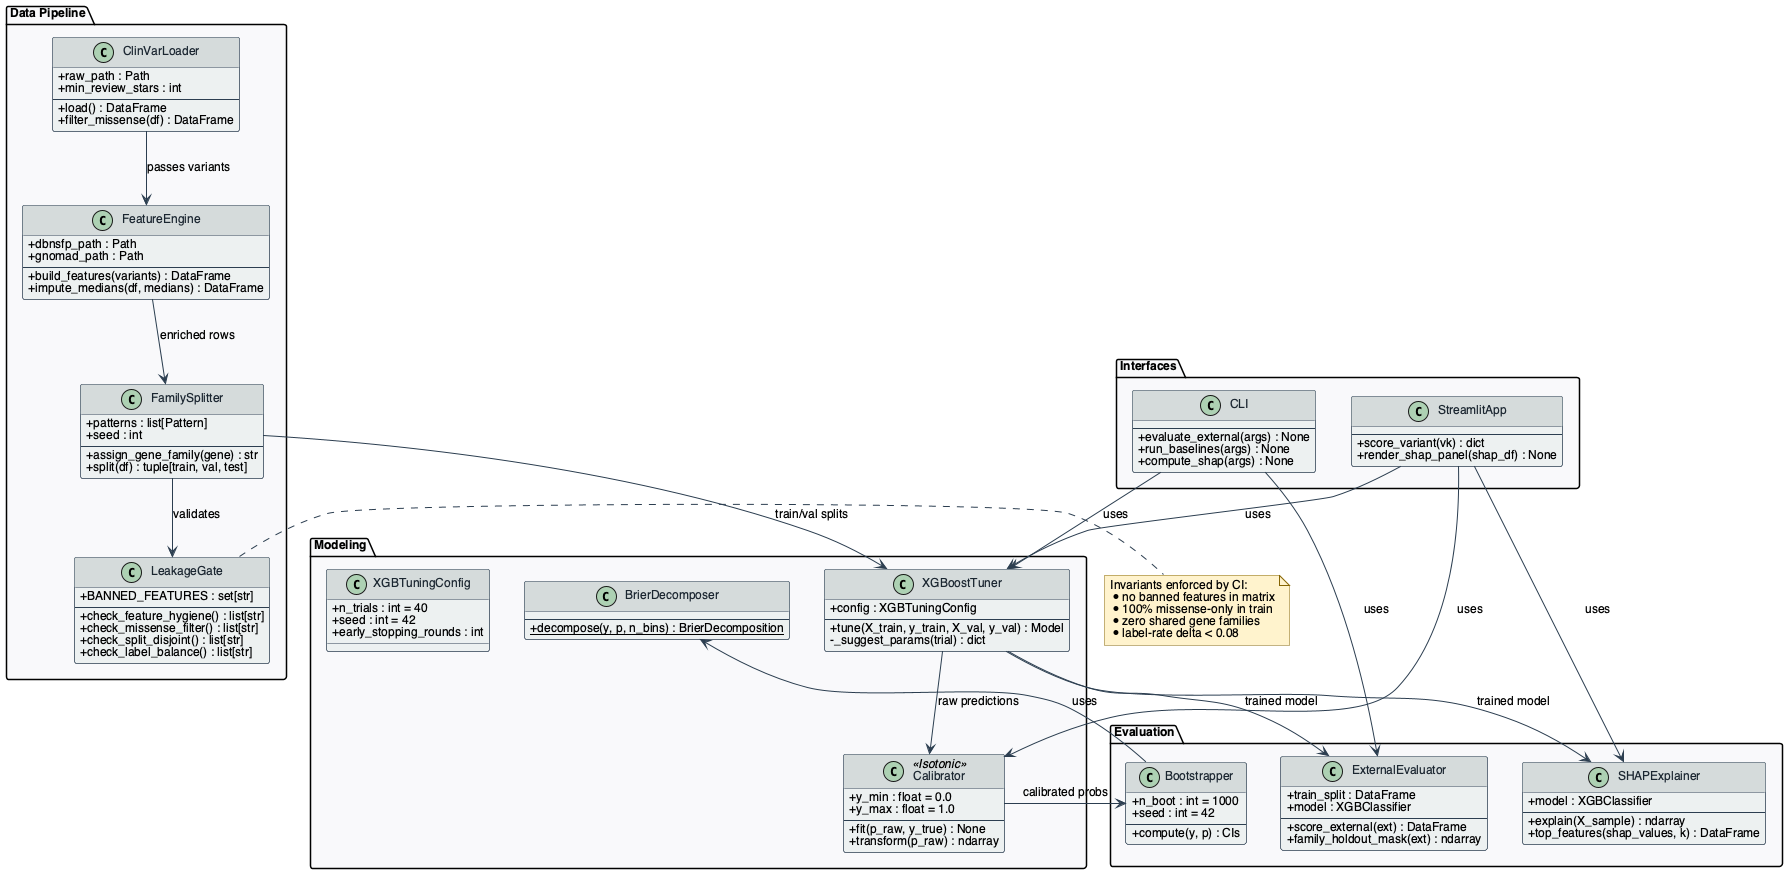
\includegraphics[width=\linewidth,height=0.78\textheight,keepaspectratio]{figures/uml/02_class.png}
  \end{columns}
\end{frame}

% ───────────── SLIDE 23 ─────────────
\begin{frame}{UML 2/3: Sequence + Activity}
  \begin{columns}[t]
    \column{0.5\linewidth}
    \centering
    \textbf{Sequence diagram}\\[0.3em]
    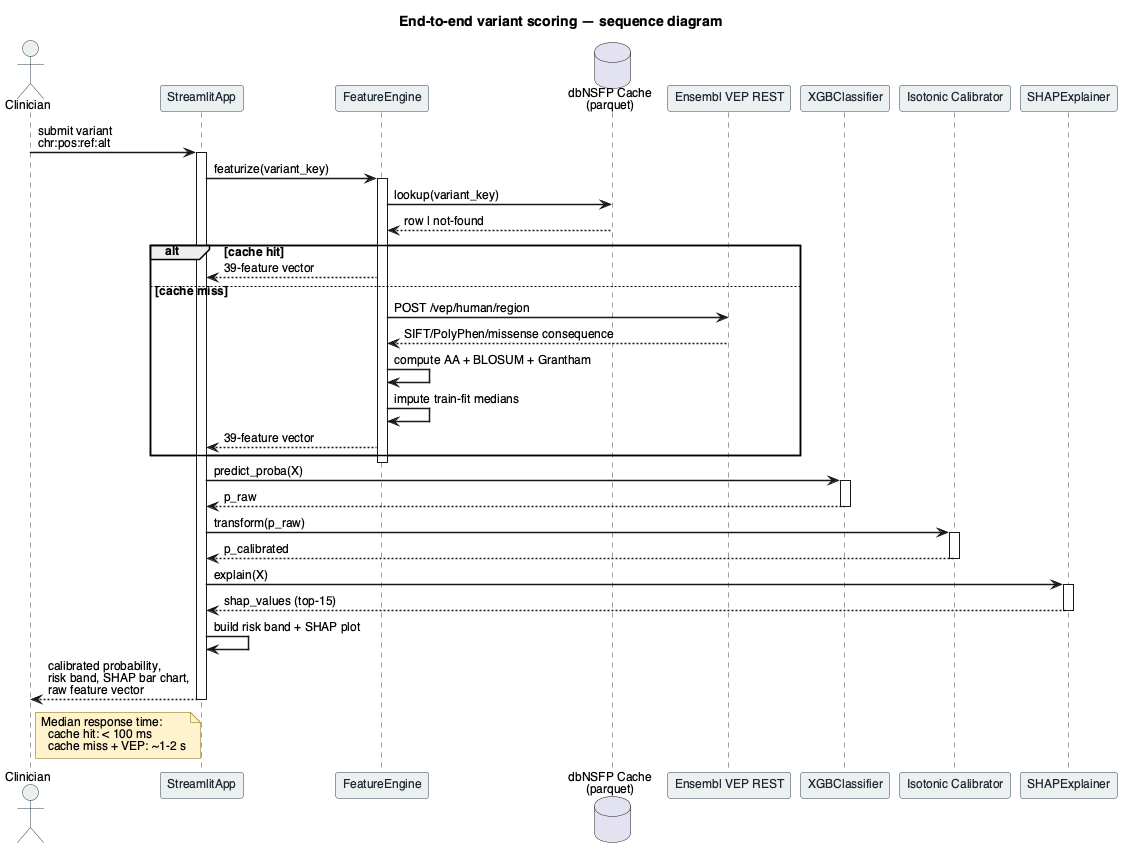
\includegraphics[width=\linewidth,height=0.78\textheight,keepaspectratio]{figures/uml/03_sequence.png}

    \column{0.5\linewidth}
    \centering
    \textbf{Activity diagram}\\[0.3em]
    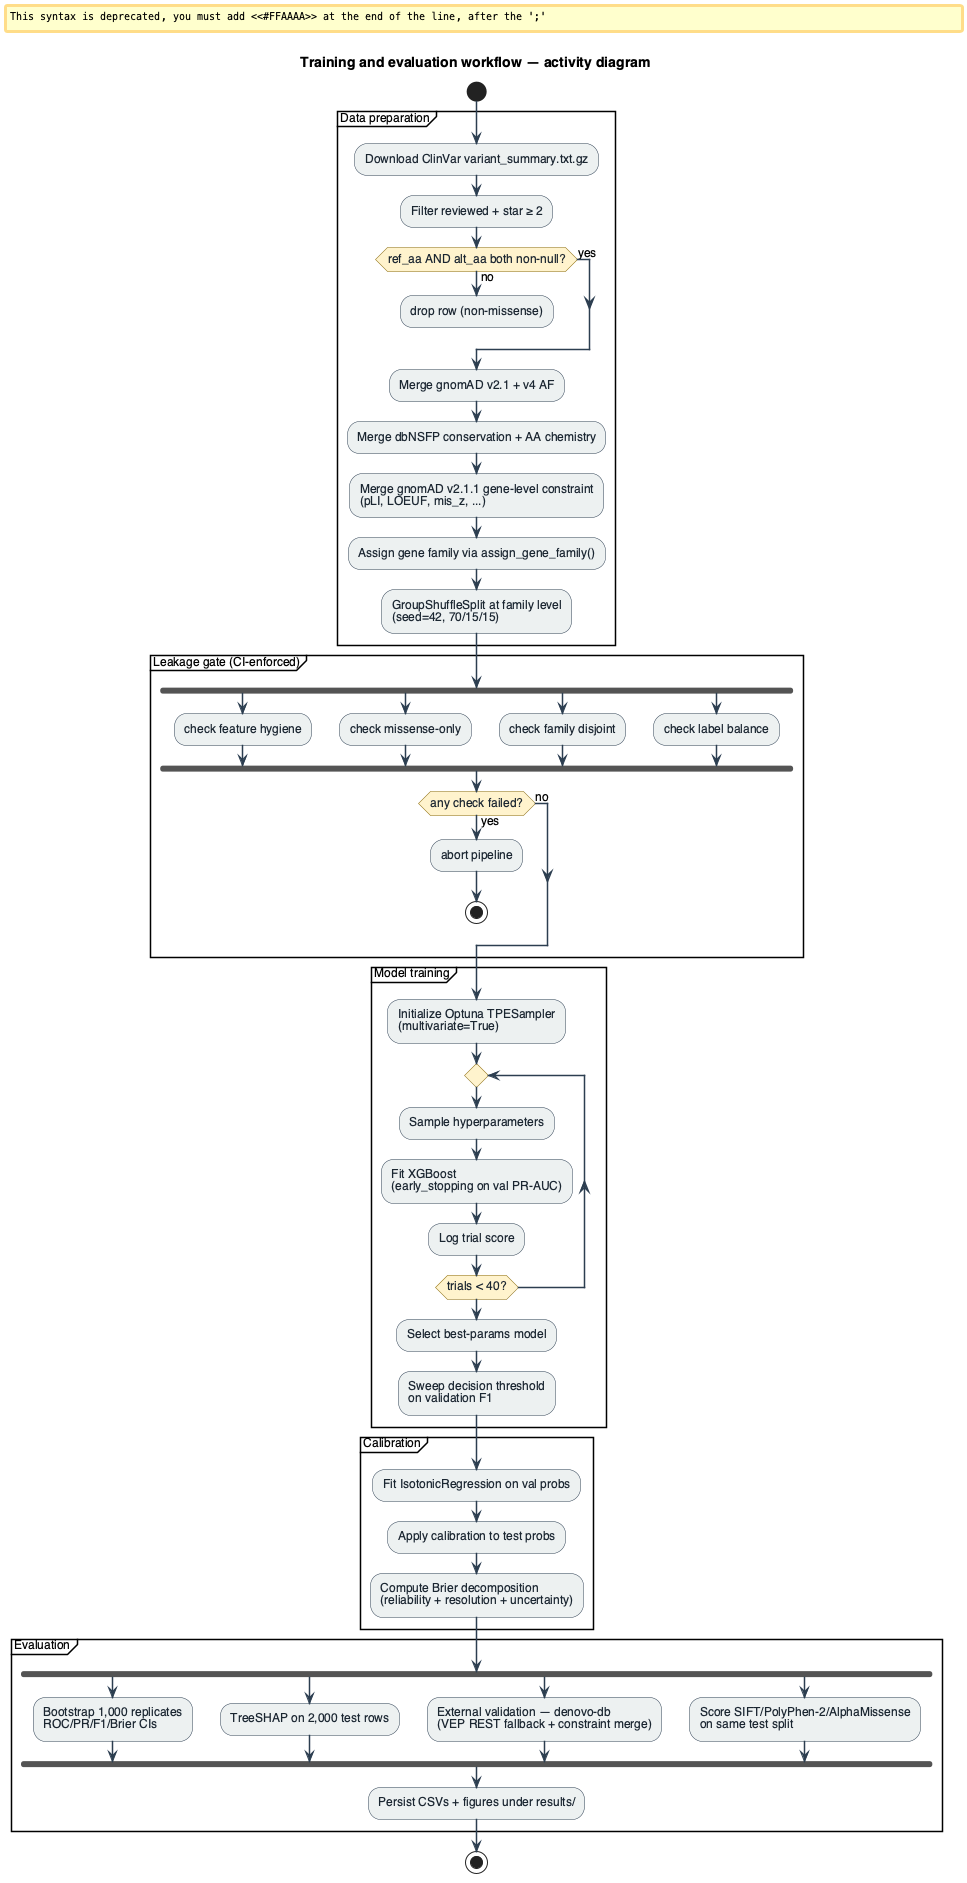
\includegraphics[width=\linewidth,height=0.78\textheight,keepaspectratio]{figures/uml/04_activity.png}
  \end{columns}
\end{frame}

% ───────────── SLIDE 24 ─────────────
\begin{frame}{UML 3/3: State + Component}
  \begin{columns}[t]
    \column{0.5\linewidth}
    \centering
    \textbf{State diagram}\\[0.3em]
    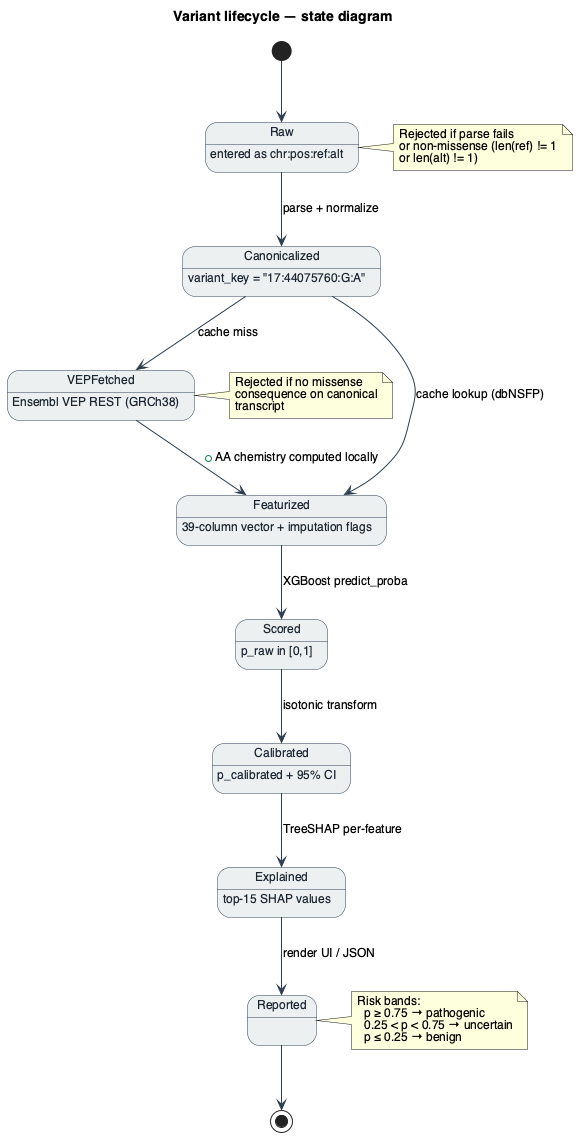
\includegraphics[width=\linewidth,height=0.78\textheight,keepaspectratio]{figures/uml/05_state.png}

    \column{0.5\linewidth}
    \centering
    \textbf{Component diagram}\\[0.3em]
    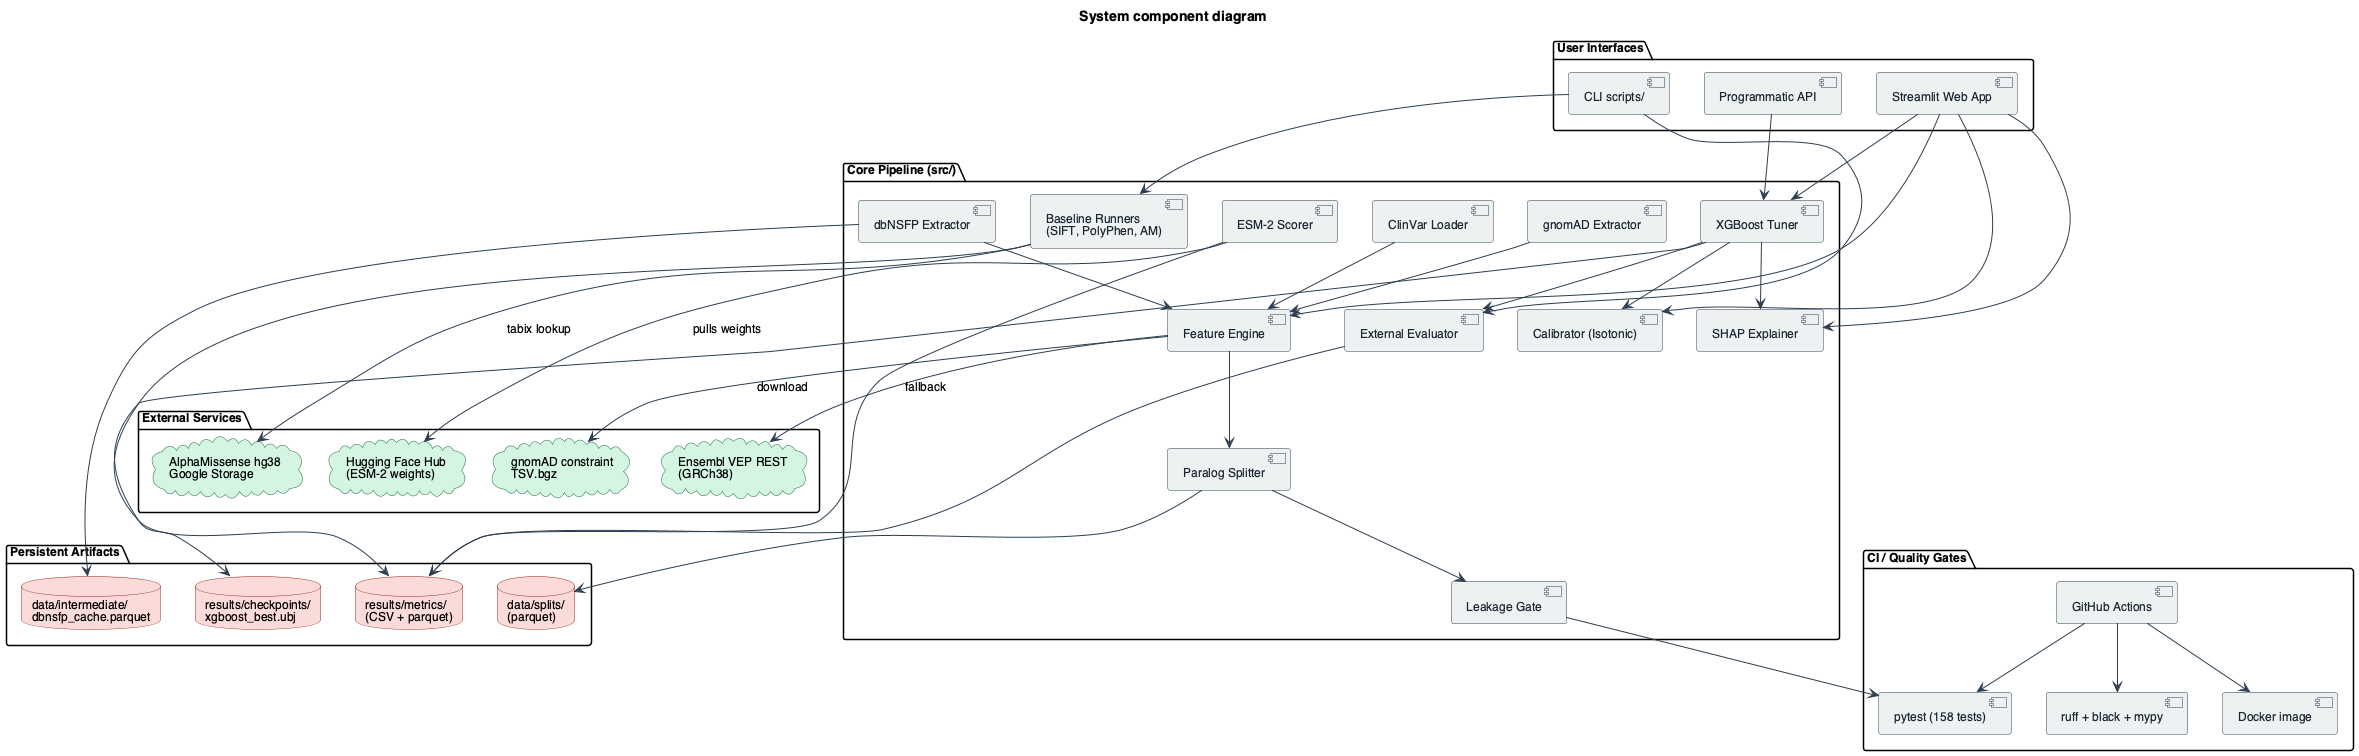
\includegraphics[width=\linewidth,height=0.78\textheight,keepaspectratio]{figures/uml/06_component.png}
  \end{columns}
\end{frame}

% ───────────── SLIDE 25 ─────────────
\begin{frame}{System architecture}
  \centering
  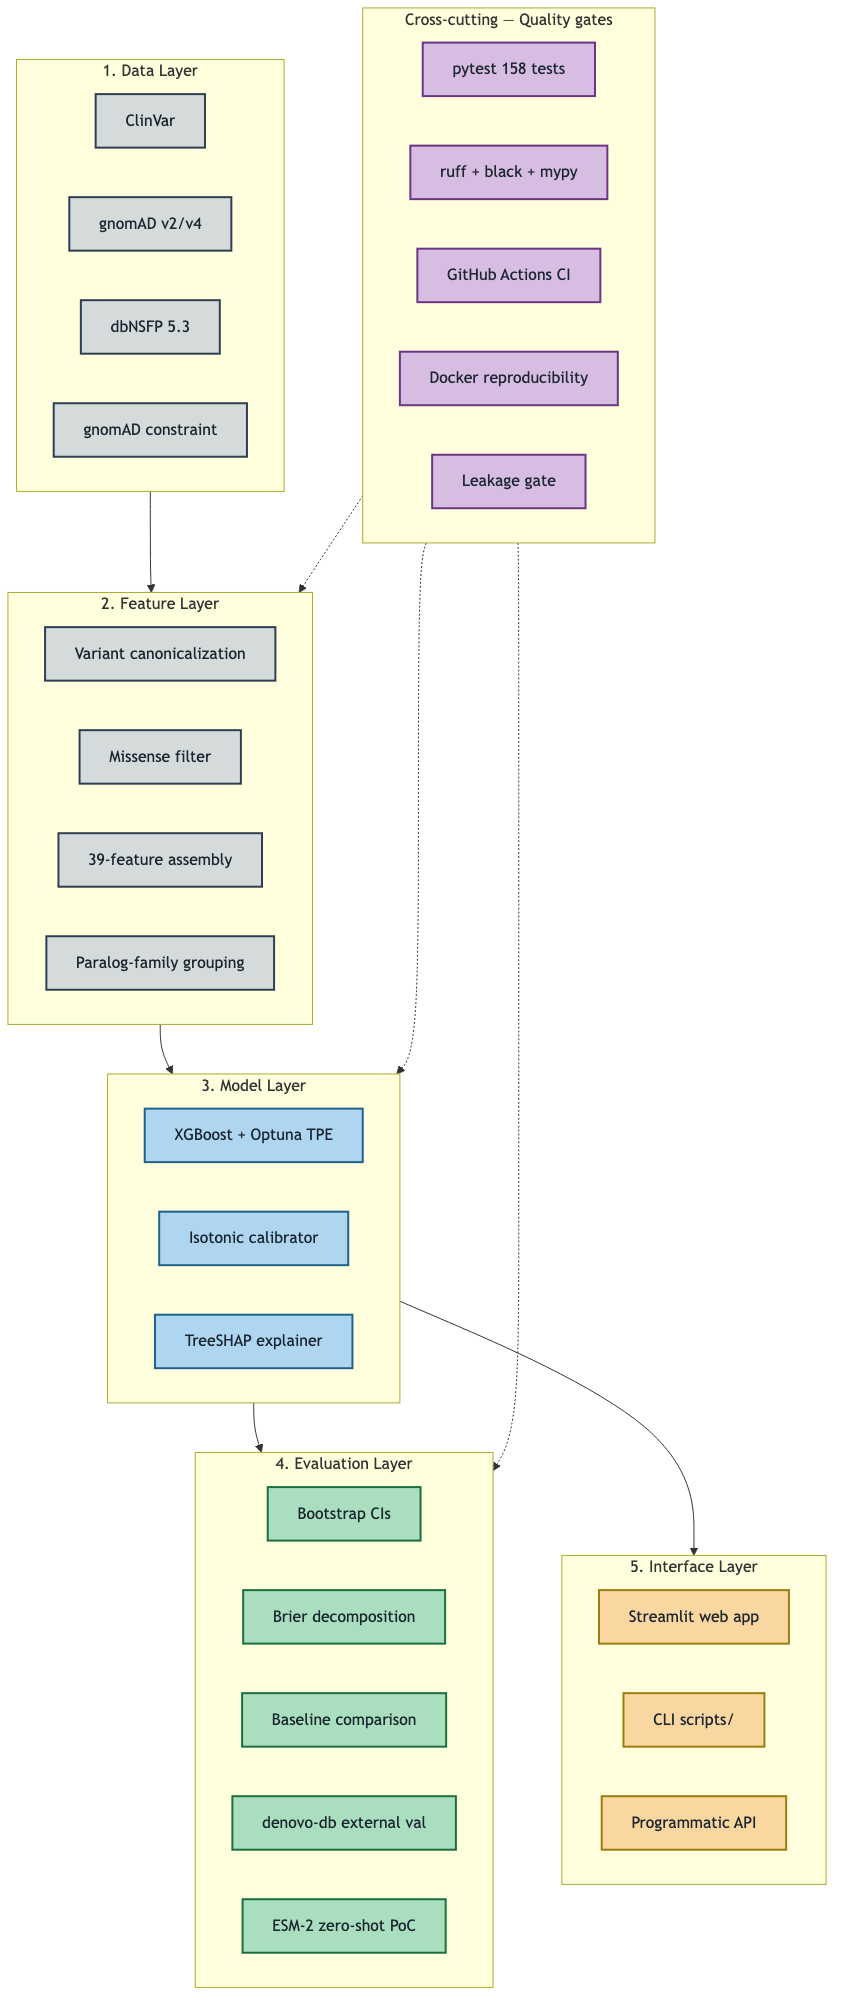
\includegraphics[width=\linewidth,height=0.82\textheight,keepaspectratio]{figures/misc/architecture.png}
\end{frame}

% ═════════════════ PART 6: INTERFACE ═════════════════
\section{Interface}

% ───────────── SLIDE 26 ─────────────
\begin{frame}{Streamlit demo -- scoring a variant}
  \centering
  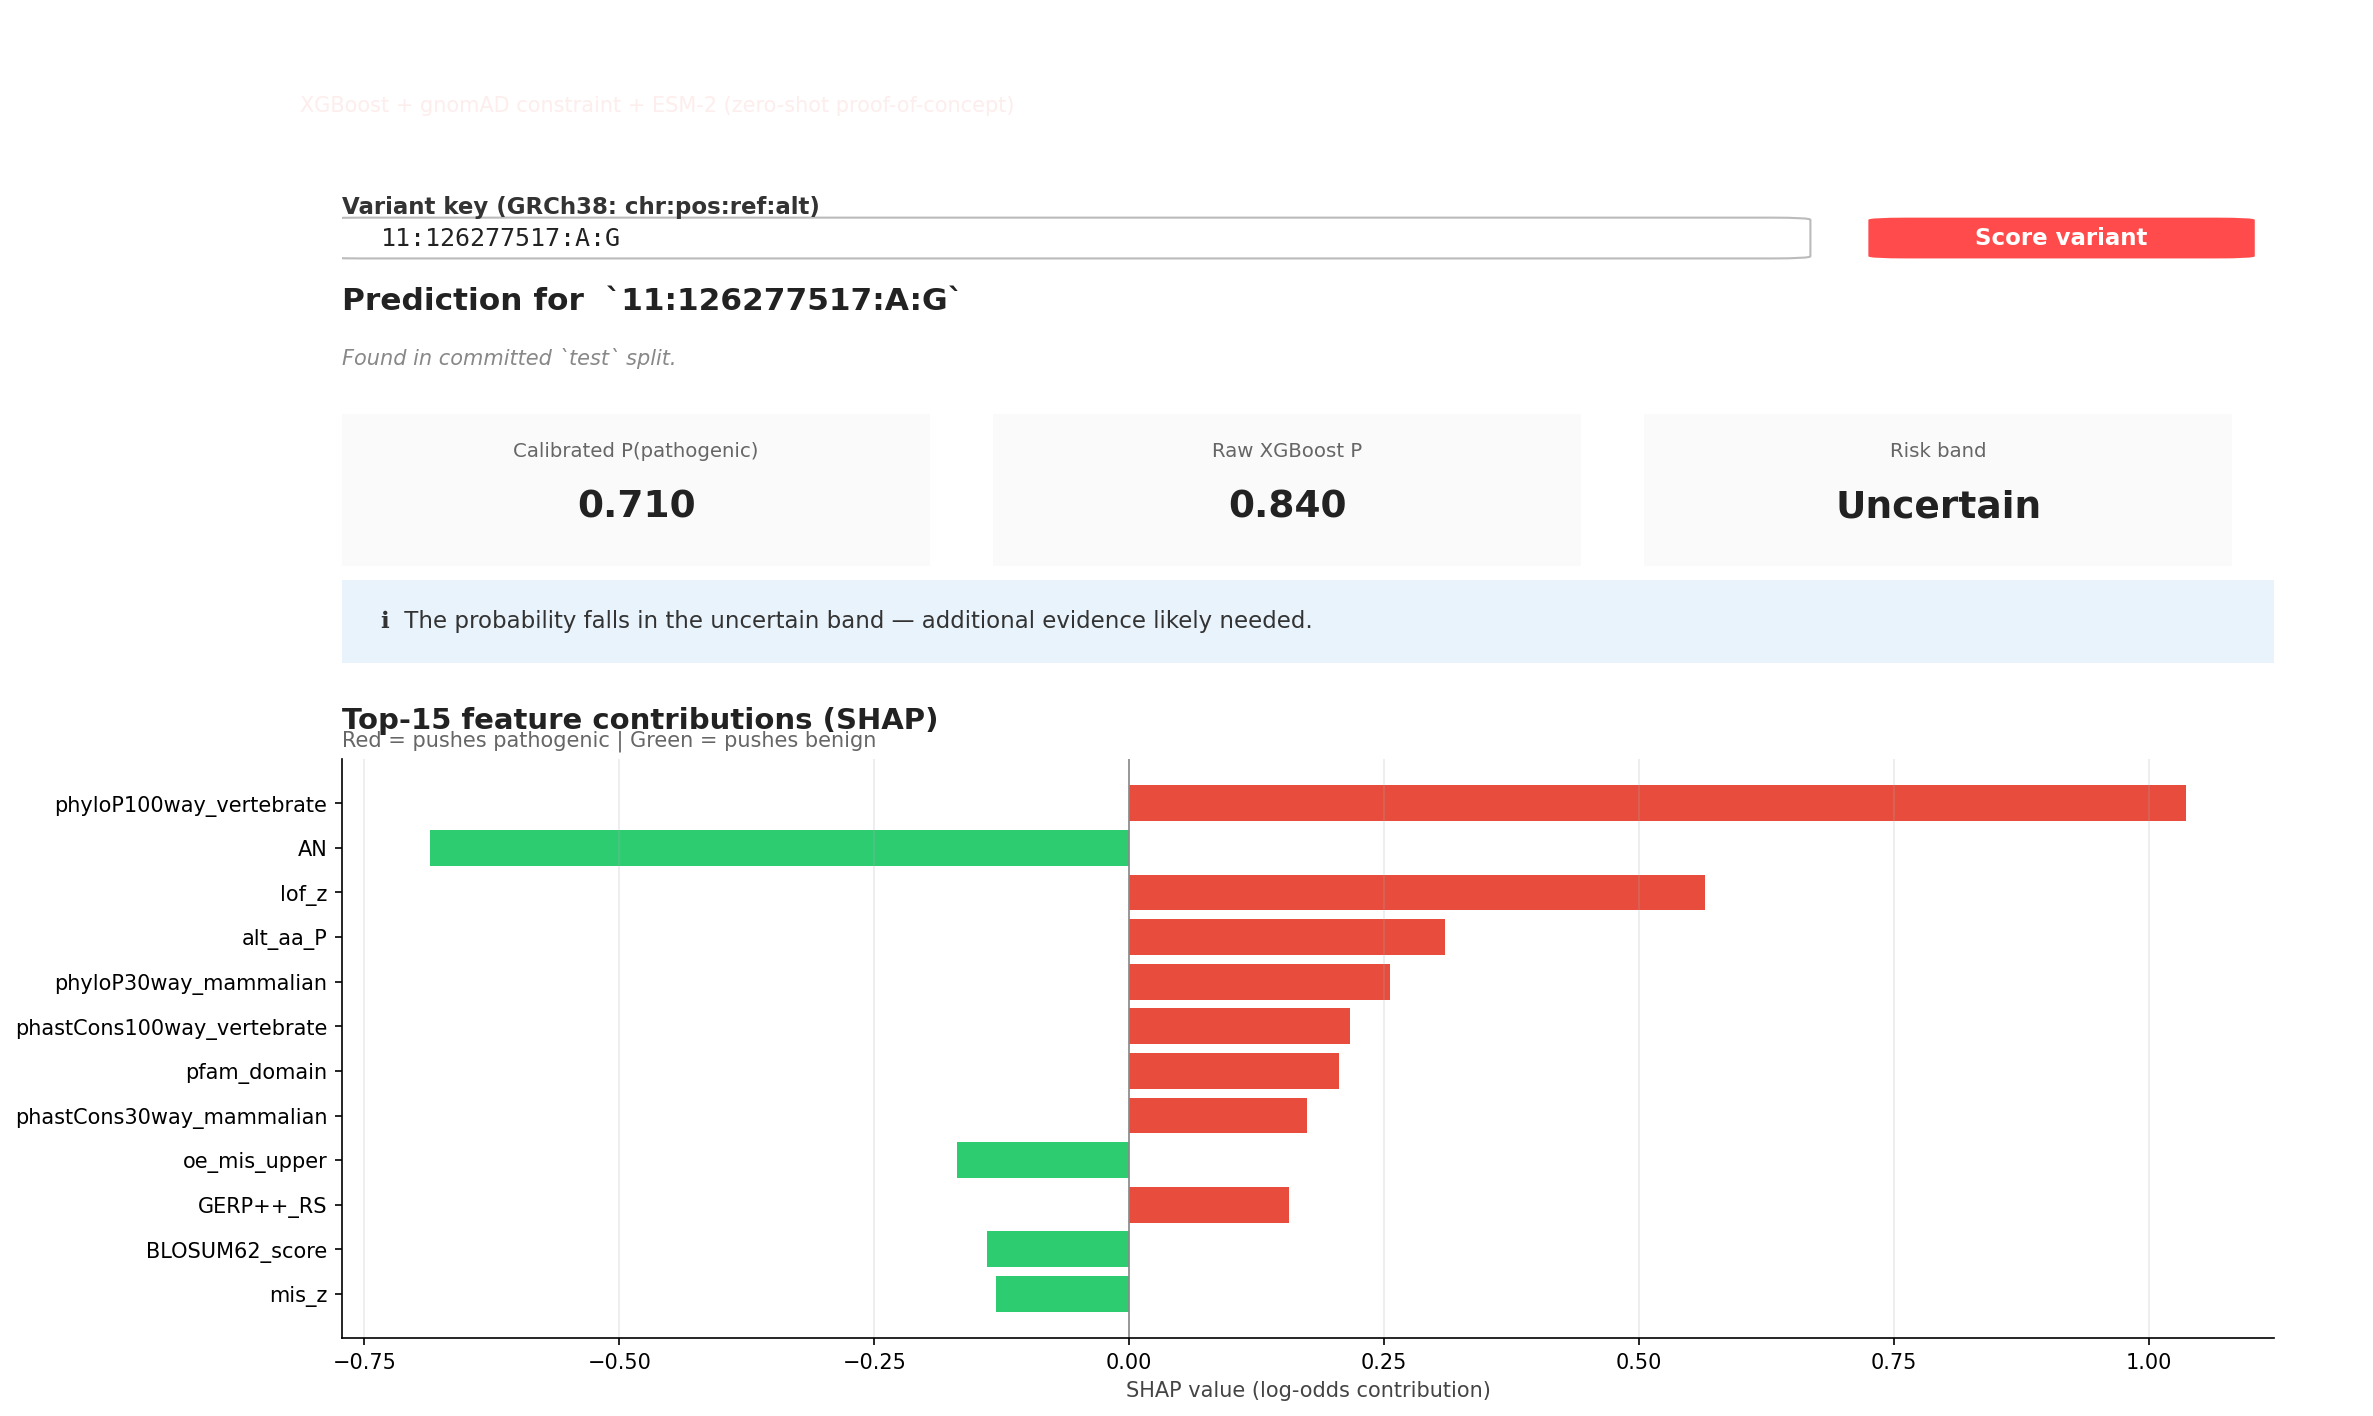
\includegraphics[width=\linewidth,height=0.82\textheight,keepaspectratio]{figures/screenshots/07_streamlit_demo.png}
\end{frame}

% ═════════════════ PART 7: IMPLEMENTATION ═════════════════
\section{Implementation}

% ───────────── SLIDE 27 ─────────────
\begin{frame}{Hardware + software stack}
  \begin{columns}[t]
    \column{0.5\linewidth}
    \textbf{Hardware}
    \begin{itemize}
      \item Apple Silicon laptop (MPS)
      \item Colab T4 GPU (Phase 2.1 only)
      \item GitHub Actions \texttt{ubuntu-22.04}
    \end{itemize}

    \column{0.5\linewidth}
    \textbf{Stack}
    \begin{itemize}
      \item Python 3.11, pinned deps
      \item XGBoost + Optuna + SHAP
      \item \texttt{transformers} + PyTorch
      \item Docker + Makefile + pre-commit
      \item 158 pytest tests, 55\%+ coverage
      \item CI: ruff + black + mypy
    \end{itemize}
  \end{columns}
\end{frame}

% ───────────── SLIDE 28 ─────────────
\begin{frame}[fragile]{Code: train-only constraint imputation}
  \begin{exampleblock}{\texttt{src/gnomad\_constraint.py}}
    \small
\begin{verbatim}
def merge_constraint(variants, *, constraint, impute_medians=None):
    merged = variants.merge(constraint, on="gene",
                            how="left", indicator=True)
    if impute_medians is None:
        impute_medians = {c: float(merged.loc[merged["_merge"] == "both",
                                              c].median())
                          for c in CONSTRAINT_COLS}
    for c in CONSTRAINT_COLS:
        merged[c] = merged[c].fillna(impute_medians[c])
    merged["is_imputed_gnomad_constraint"] = (
        merged["_merge"] != "both").astype(int)
    return merged.drop(columns="_merge"), impute_medians
\end{verbatim}
  \end{exampleblock}
  \begin{itemize}
    \item Medians fit on \emph{train only} $\Rightarrow$ no leakage.
    \item Flag column exposed to SHAP for analysis.
  \end{itemize}
\end{frame}

% ───────────── SLIDE 29 ─────────────
\begin{frame}{Continuous integration: 158 tests on every push}
  \centering
  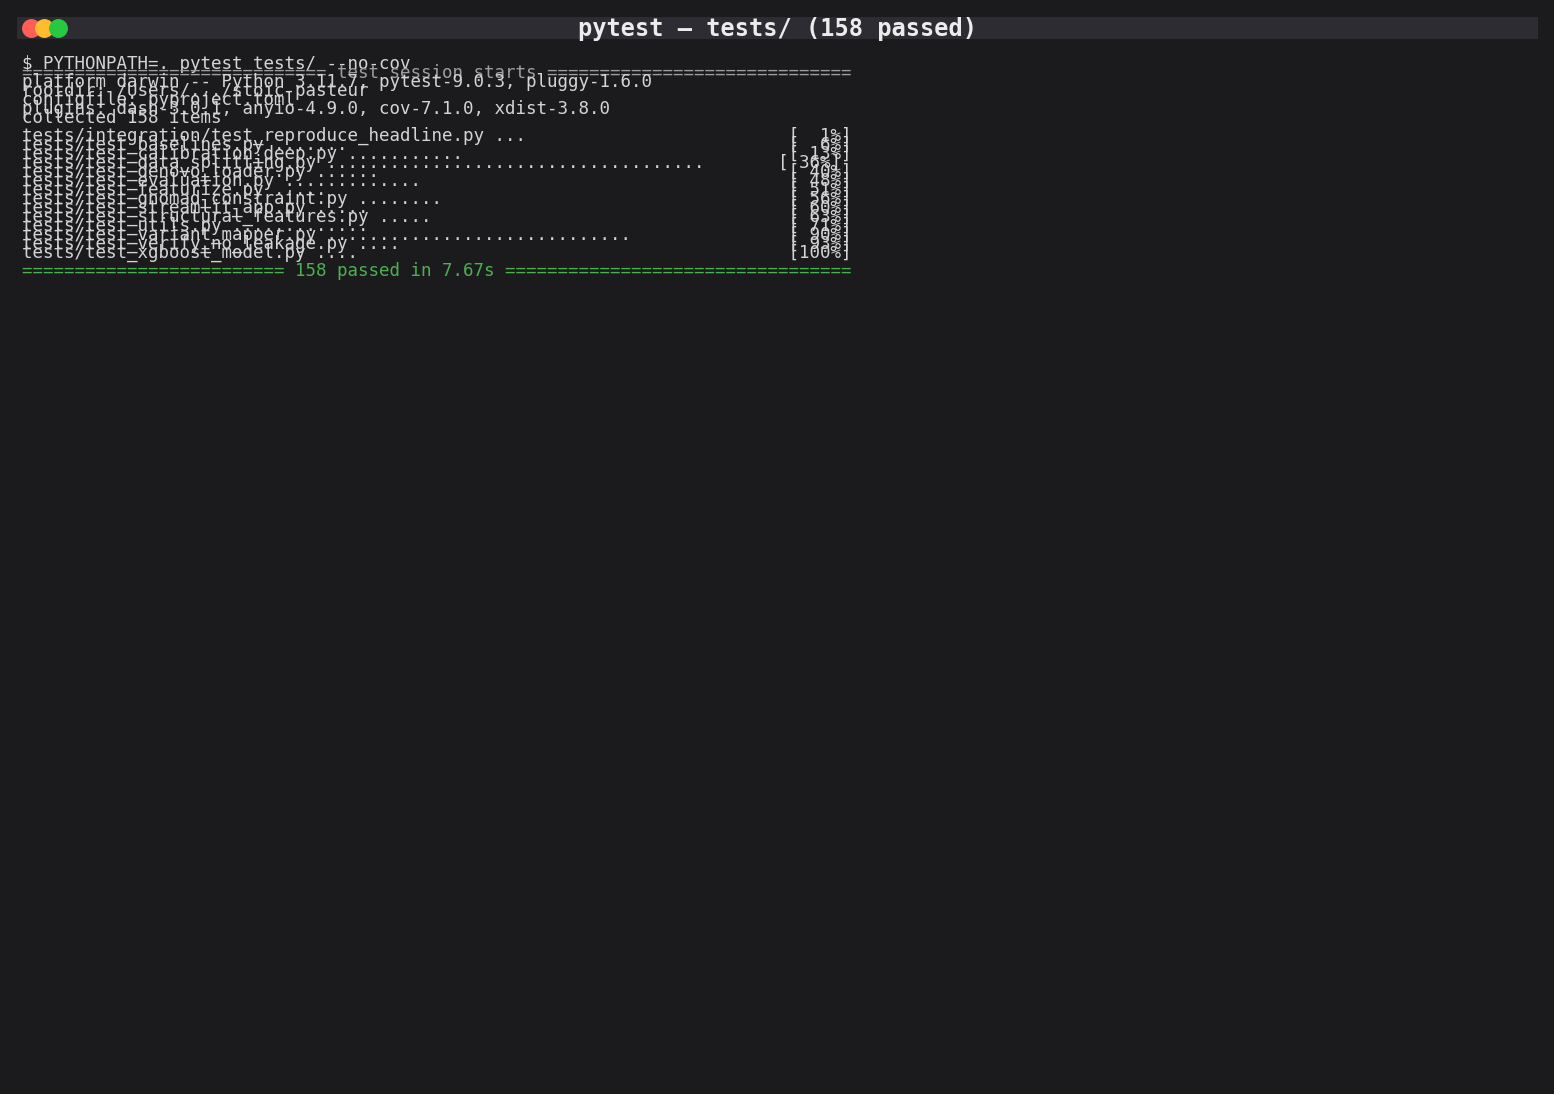
\includegraphics[width=\linewidth,height=0.68\textheight,keepaspectratio]{figures/screenshots/01_pytest_output.png}
\end{frame}

% ───────────── SLIDE 30 ─────────────
\begin{frame}{Leakage gate -- CI-enforced invariants}
  \centering
  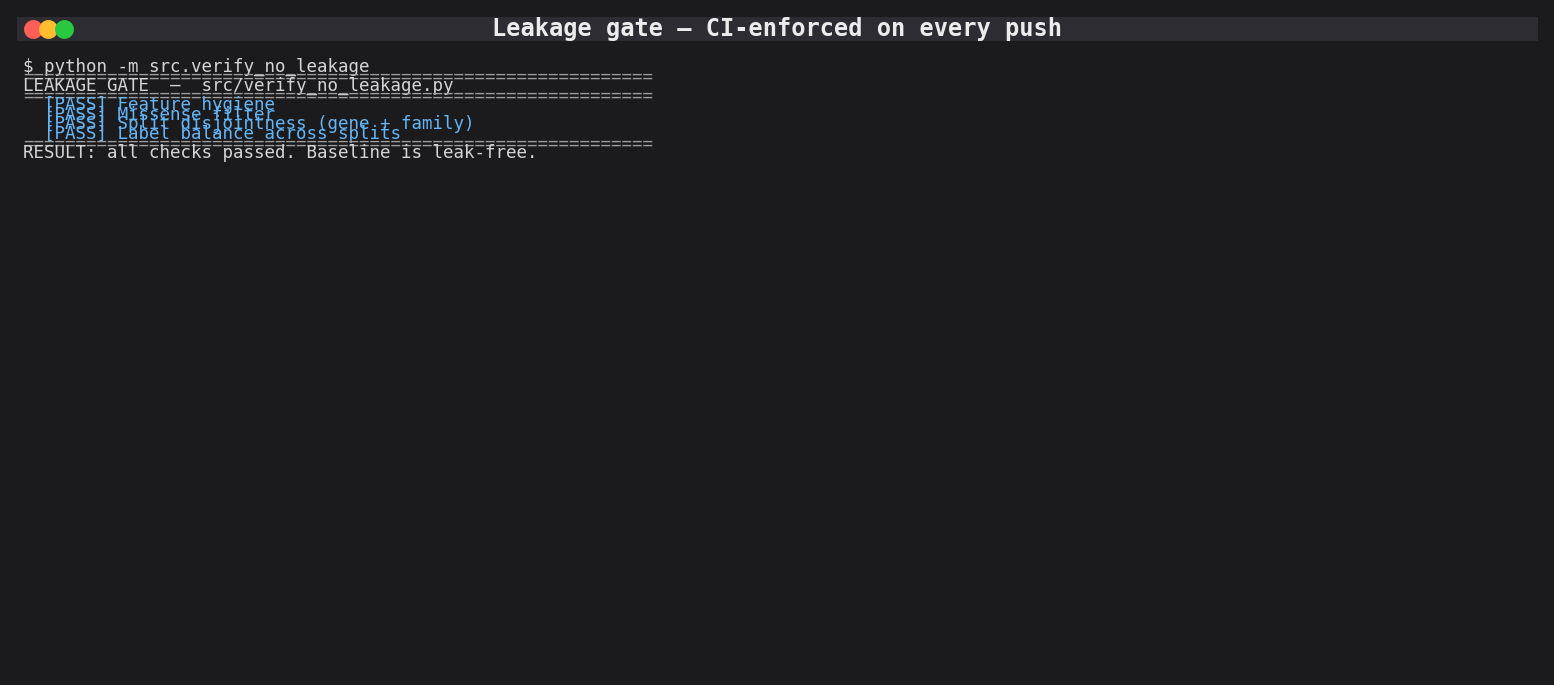
\includegraphics[width=0.78\linewidth,height=0.65\textheight,keepaspectratio]{figures/screenshots/02_leakage_gate.png}
\end{frame}

% ───────────── SLIDE 31 ─────────────
\begin{frame}{Phase 2.1 -- ESM-2 on Colab (zero-shot LLR)}
  \centering
  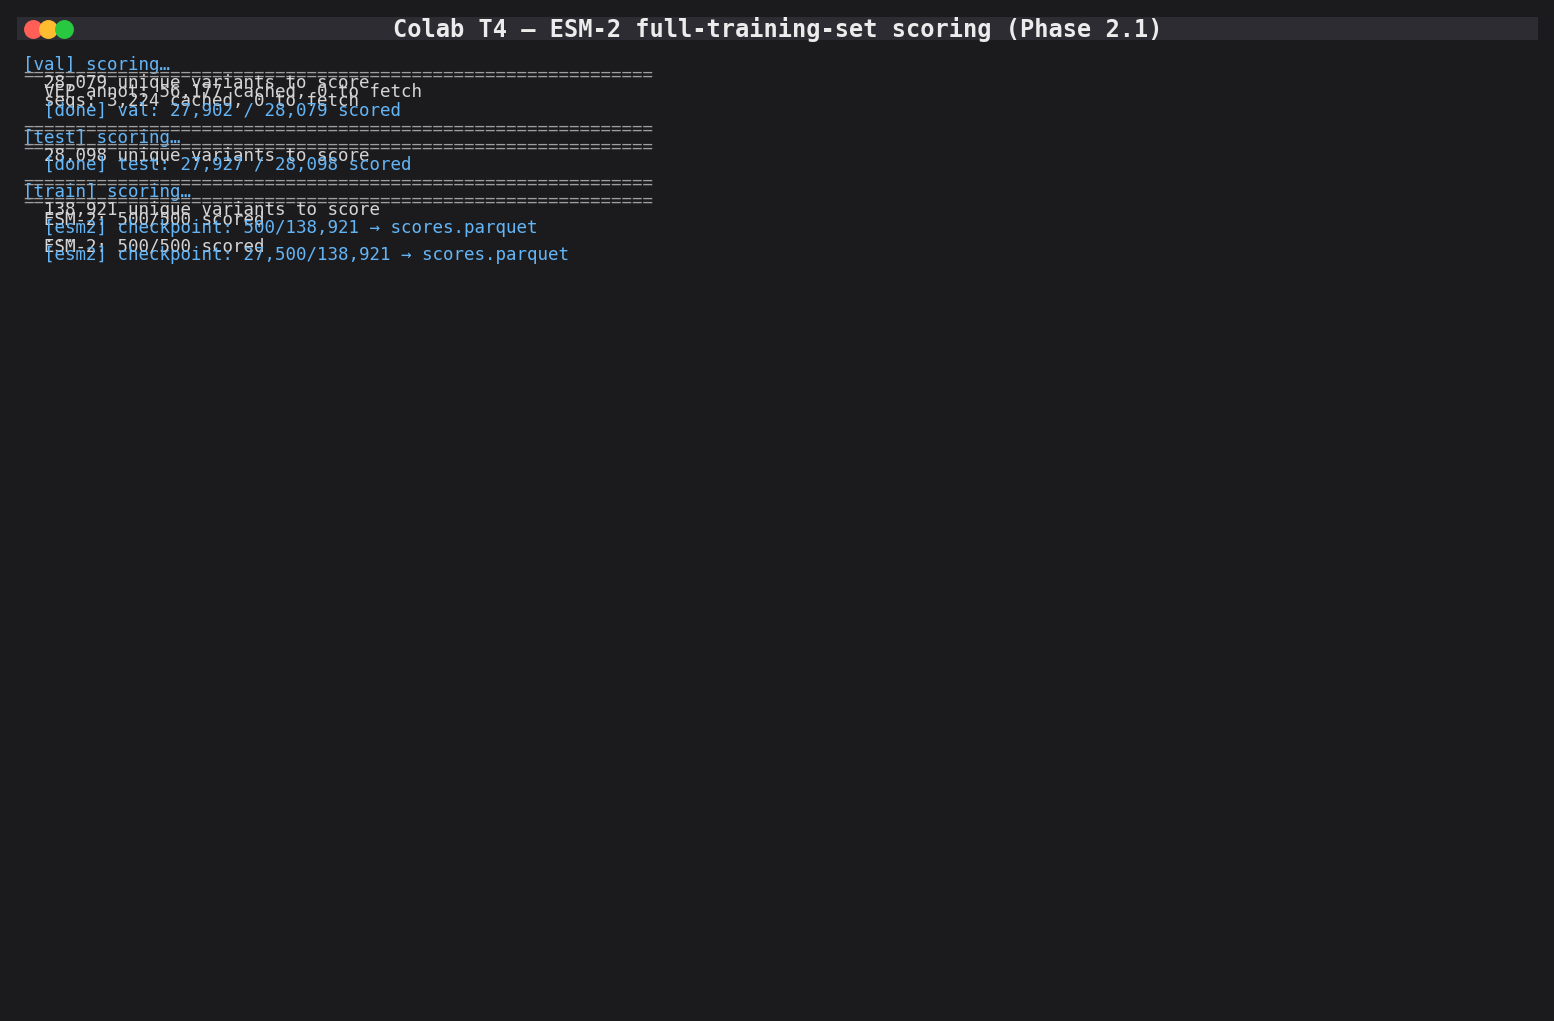
\includegraphics[width=0.85\linewidth,height=0.68\textheight,keepaspectratio]{figures/screenshots/05_colab_esm2.png}
\end{frame}

% ═════════════════ PART 8: COMPARISON ═════════════════
\section{Comparison}

% ───────────── SLIDE 32 ─────────────
\begin{frame}{Comparison on our test split}
  \centering
  \textbf{Identical evaluation: paralog-disjoint test (28{,}098 variants)}
  \vspace{0.4em}
  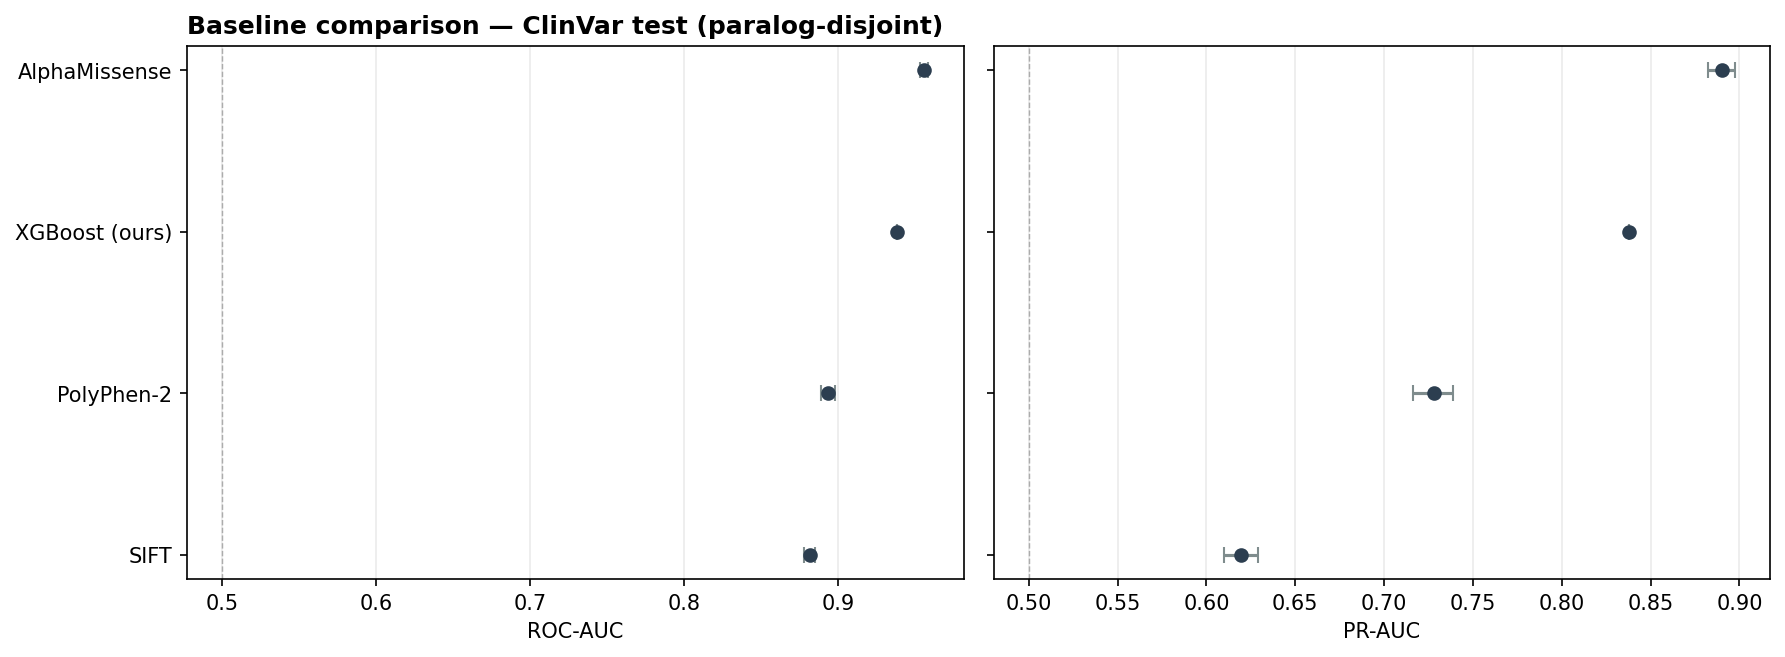
\includegraphics[width=\linewidth,height=0.66\textheight,keepaspectratio]{figures/scientific/baselines_forest_plot.png}
  \vspace{0.4em}
  \begin{itemize}
    \item $+0.22$ PR-AUC over SIFT, $+0.11$ over PolyPhen-2.
    \item $-0.05$ below AlphaMissense (\alert{calibrated on ClinVar}).
  \end{itemize}
\end{frame}

% ═════════════════ PART 9: CONCLUSION ═════════════════
\section{Conclusion}

% ───────────── SLIDE 33 ─────────────
\begin{frame}{Take-home messages}
  \begin{enumerate}
    \item \textbf{Audited numbers beat inflated ones.} \\
          Our 0.838 PR-AUC has no known contamination; the pre-audit
          0.955 had three.
    \item \textbf{Like-for-like baselines change the conversation.} \\
          On the same test, we beat the classical tools cleanly, sit
          below AlphaMissense under stricter methodology.
    \item \textbf{External validation is the real benchmark.} \\
          At chance on denovo-db without gene priors, above chance
          after --- and this is the diagnostic that motivates Phase 2.
  \end{enumerate}
\end{frame}

% ───────────── SLIDE 34 ─────────────
\begin{frame}{Future work (Phase 2)}
  \begin{enumerate}
    \item \textbf{ESM-2 full-training-set integration.} \\
          Zero-shot PoC shows $+0.015$ ROC from rank fusion. Full
          compute running on Colab T4.
    \item \textbf{AlphaFold2 structural features.} \\
          pLDDT, SASA, DSSP secondary structure, residue depth.
    \item \textbf{ProteinGym external validation.} \\
          Third external dataset (deep mutational scanning).
    \item \textbf{Hybrid stacking + clinical integration.} \\
          Meta-learner + ACMG-compatible plug-in.
  \end{enumerate}
\end{frame}

% ───────────── SLIDE 35 ─────────────
\begin{frame}[plain]{}
  \vspace{1.4cm}
  \centering
  \huge Thank you.
  \vspace{0.8em}

  \Large Questions?
  \vspace{1.4cm}

  \normalsize
  \begin{tabular}{@{} l @{}}
    Code, tests, Docker, notebooks, report, slides: \\[0.4em]
    \small \url{github.com/RayanAlDwlah/Genetic-Mutation-Detection-project}
  \end{tabular}
\end{frame}

\end{document}
